\section{Iterations} 

\subsection{Project Sprints}

\begin{table}[!hbt]
\centering
\caption{Overview metrics for all 3 sprints.}
\label{tab: overview table}
\begin{tabular}{|c|c|c|c|c|}
\hline
\textbf{Sprint \#} &
  \textbf{Remainder (pts)} &
  \textbf{Planned (pts)} &
  \textbf{\begin{tabular}[c]{@{}c@{}}Completed (pts)\\ (Speed)\end{tabular}} &
  \textbf{\begin{tabular}[c]{@{}c@{}}Cycle\\ (hrs/pts)\end{tabular}} \\ \hline
Sprint 1 & 39 & 12 & 8  & 17.4 \\ \hline
Sprint 2 & 31 & 21 & 21 & 5.9  \\ \hline
Sprint 3 & 10 & 10 & 10 & 9.2  \\ \hline
\end{tabular}
\end{table}

\noindent Table \ref{tab: overview table} shows the progression of each sprint in terms of story points. The first column shows all the points left to be completed, thus in sprint 1 that would be all points in the whole project. The second column shows the ones that we as a team planned to accomplish for that sprint, while the third column shows those that were actually completed and approved by the end of that sprint. The fourth column expresses the time as a function of total hours $\div$ the total points (not including technical tasks or spikes) for that sprint.

\subsection{Sprint 1}

\subsubsection{Plan}
In this sprint we aimed to get a simple working version of Blackjack that runs from a GUI.

\noindent We added 6 (Main, card, deck, hand, player, and game).java that serves as our business logic for our game. Additionally we added a login screen that allows the user to sign in, create an account, or play as a guest. We have also implemented the base for our backend database that stores our users login info.

\subsubsection{Sprint 1 Stories}

\begin{table}[!hbt]
\centering
\caption{Overview for sprint 1}
\label{tab: sprint 1 overview}
\begin{tabular}{|c|c|c|c|c|}
\hline
\textbf{ID} & \textbf{Name}  & \textbf{Points} & \textbf{Contributor} & \textbf{Status}                       \\ \hline
S1          & Login          & 2               & Jenna / Emma         & {\color[HTML]{32CB00} Accepted}       \\ \hline
S2          & Logout         & 1               & Jenna / Emma         & {\color[HTML]{CB0000} Unaccomplished} \\ \hline
S3          & Create Account & 2               & Jenna / Emma         & {\color[HTML]{32CB00} Accepted}       \\ \hline
S7          & Play as Guest  & 2               & Jenna / Emma         & {\color[HTML]{CB0000} Unaccomplished} \\ \hline
S14         & Hit            & 1               & Chris / Callie       & {\color[HTML]{FFCB2F} Superseded}     \\ \hline
S21         & View Tutorial  & 1               & Chris / Callie       & {\color[HTML]{32CB00} Accepted}       \\ \hline
S26         & Play Blackjack & 3               & Chris / Callie       & {\color[HTML]{32CB00} Accepted}       \\ \hline
\end{tabular}
\end{table}

\noindent Table \ref{tab: sprint 1 overview} shows the overview for the first sprint. It shows the stories that were attempted A unique dynamic to sprint 1 was that we used paired programming (shown in the Contributor column) to start our project. This was so that we all got off on the right foot and could start this project on the same page. Another thing worth noting is that in the Status column, some stories are set as unaccomplished. This means that we as a team did not think that the story was ready for the acceptance test, not that our client did not accept the story. Lastly, S14 was superseded, meaning that we did not believe that story rose to the level of a true user story, thus we set it as superseded and it was incorporated into S26 - play blackjack.

\begin{table}[!hbt]
\centering
\caption{Individual metrics for sprint 1}
\label{tab: sprint 1 individual metrics}
\begin{tabular}{|c|c|c|c|c|c|}
\hline
\textbf{Name} &
  \textbf{\begin{tabular}[c]{@{}c@{}}Points\\ Attempted\end{tabular}} &
  \textbf{\begin{tabular}[c]{@{}c@{}}Points\\ Completed\\ (Speed)\end{tabular}} &
  \textbf{\begin{tabular}[c]{@{}c@{}}Paired \\ Programming\\ ($\div 2$)\end{tabular}} &
  \textbf{\begin{tabular}[c]{@{}c@{}}Work \\ (hrs)\end{tabular}} &
  \textbf{\begin{tabular}[c]{@{}c@{}}Cycle\\ (hrs/pts)\end{tabular}} \\ \hline
Chris  & 5 & 4 & 2 & 35 & 16   \\ \hline
Jenna  & 7 & 4 & 2 & 40 & 20   \\ \hline
Callie & 5 & 4 & 2 & 35 & 17.5 \\ \hline
Emma   & 7 & 4 & 2 & 29 & 14.5 \\ \hline
\end{tabular}
\end{table}

\noindent Table \ref{tab: sprint 1 individual metrics} shows the individual metrics for sprint 1. As mentioned before, this sprint incorporated paired programming which takes the individual speeds and divides them by 2 thus giving each individual a speed of column 3 $\div 2$ = column 4. This number was the speed taken into account when determining each individual's cycle. Something worth noting in this table is the work column. For only having 8pts, the hours shown in the work column seem very high. Since this was sprint 1, there was a lot of overhead and setting up required to start this project thus giving us very high . We didn't do a good job of documenting things like technical tasks or spikes in this sprint which is explained more in the retrospective for this sprint down below. 

\subsubsection{Sprint 1 Testing}

Here are the individual testing results for each member:

\begin{table}[!hbt]
\centering
\caption{Sprint 1 testing coverage by main contributor}
\label{tab: sprint 1 testing}
\begin{tabular}{|ccc|}
\hline
\multicolumn{1}{|c|}{\textbf{File}}                                              & \multicolumn{1}{c|}{\textbf{Statement Coverage (\%)}} & \textbf{Branch Coverage (\%)} \\ \hline
\multicolumn{3}{|c|}{\textbf{Chris}}                                                                                                 \\ \hline
\multicolumn{1}{|c|}{Card}                                                      & \multicolumn{1}{c|}{100}           & 100           \\ \hline
\multicolumn{1}{|c|}{Deck}                                                      & \multicolumn{1}{c|}{100}           & 100           \\ \hline
\multicolumn{1}{|c|}{Game}                                                      & \multicolumn{1}{c|}{80}            & 70            \\ \hline
\multicolumn{1}{|c|}{Hand}                                                      & \multicolumn{1}{c|}{97}            & 93            \\ \hline
\multicolumn{1}{|c|}{Player}                                                    & \multicolumn{1}{c|}{100}           & 100           \\ \hline
\multicolumn{1}{|c|}{\textbf{Average}}                                          & \multicolumn{1}{c|}{\textbf{95.4}} & \textbf{92.6} \\ \hline
\multicolumn{3}{|c|}{\textbf{Jenna}}                                                                                                 \\ \hline
\multicolumn{1}{|c|}{\begin{tabular}[c]{@{}c@{}}User\\ Controller\end{tabular}} & \multicolumn{1}{c|}{74}            & 62            \\ \hline
\multicolumn{1}{|c|}{\begin{tabular}[c]{@{}c@{}}Logout\\ Controller\end{tabular}} & \multicolumn{1}{c|}{100}                              & 100                           \\ \hline
\multicolumn{1}{|c|}{\textbf{Average}}                                          & \multicolumn{1}{c|}{\textbf{87}}   & \textbf{81}   \\ \hline
\multicolumn{3}{|c|}{\textbf{Callie}}                                                                                                \\ \hline
\multicolumn{1}{|c|}{\begin{tabular}[c]{@{}c@{}}Game\\ Controller\end{tabular}} & \multicolumn{1}{c|}{91}            & 77            \\ \hline
\multicolumn{1}{|c|}{\textbf{Average}}                                          & \multicolumn{1}{c|}{\textbf{91}}   & \textbf{77}   \\ \hline
\multicolumn{3}{|c|}{\textbf{Emma}}                                                                                                  \\ \hline
\multicolumn{1}{|c|}{App/page}                                                  & \multicolumn{1}{c|}{100}           & 100           \\ \hline
\multicolumn{1}{|c|}{\textbf{Average}}                                          & \multicolumn{1}{c|}{\textbf{100}}  & \textbf{100}  \\ \hline
\end{tabular}
\end{table}

\noindent Table \ref{tab: sprint 1 testing} shows the testing for all the files developed in sprint 1 grouped by primary contributor. Some stand out data including the low coverage for Game, User controller and Game controller can be attributed to the complexity of those files. For the Game file, the blackjack game itself has a lot of edge cases that are easy to miss because of their infrequency in the game. For the User controller and the Game controller, the endpoint testing is what caused the low testing coverage. 

\subsubsection{Sprint 1 Retrospective}
In sprint 1 we had quite the eye opening experience as to how complicated creating a project of this magnitude can be. We realized that infrequent integration between components such as model, view and controller is much harder and can produce more problems than we thought. Additionally, our biggest epiphany was that our original point values for our user stories were considerably underestimated with the highest point value story in the project being 3pts. 

\subsection{Sprint 2}


\subsubsection{Plan}

\noindent Our plan for sprint 2 was to develop the social aspects of the game around a simple single-player version of our game. This included more robust sign in/out, guest user handling, messaging and friend management. Additionally, we aimed to start to create the lobby components of the app including the table list and the information about each table.

\subsubsection{Sprint 2 Stories}

\begin{table}[!hbt]
\centering
\caption{Overview for sprint 2}
\label{tab: sprint 2 overview}
\begin{tabular}{|c|c|c|c|c|}
\hline
\textbf{ID} & \textbf{Name}                                                        & \textbf{Points} & \textbf{Contributor} & \textbf{Status}                       \\ \hline
S2          & Logout                                                               & 1               & Jenna                & {\color[HTML]{32CB00} Accepted}       \\ \hline
S4          & View Friends List                                                    & 1               & Jenna                & {\color[HTML]{32CB00} Accepted} \\ \hline
S5          & Add Friend                                                           & 1               & Jenna                & {\color[HTML]{32CB00} Accepted}       \\ \hline
S6          & Remove Friend                                                        & 1               & Jenna                & {\color[HTML]{CB0000} Unaccomplished} \\ \hline
S7          & Play as Guest                                                        & 2               & Jenna                & {\color[HTML]{32CB00} Accepted}       \\ \hline
S8          & Create Table                                                         & 2               & Chris                & {\color[HTML]{32CB00} Accepted}       \\ \hline
S9          & {\color[HTML]{FFC702} View Table Info}                               & 2               & Chris                & {\color[HTML]{32CB00} Accepted}       \\ \hline
S10         & Join Table                                                           & 2               & Chris                & {\color[HTML]{32CB00} Accepted}       \\ \hline
S11         & {\color[HTML]{FFC702} Leave Table}                                   & 2               & Chris                & {\color[HTML]{32CB00} Accepted}       \\ \hline
S12         & Join Game                                                            & 2               & Chris                & {\color[HTML]{CB0000} Unaccomplished} \\ \hline
S15         & Change Ace Value                                                     & 1               & Callie               & {\color[HTML]{CB0000} Unaccepted}     \\ \hline
S19         & View Game History                                                    & 2               & Emma                 & {\color[HTML]{32CB00} Accepted}       \\ \hline
S20         & Buy Chips                                                            & 2               & Emma                 & {\color[HTML]{32CB00} Accepted}       \\ \hline
S22 & \begin{tabular}[c]{@{}c@{}}Send Message \\ to Admin\end{tabular}              & 2 & Callie & {\color[HTML]{32CB00} Accepted} \\ \hline
S23 & \begin{tabular}[c]{@{}c@{}}Send Message \\ to Friend\end{tabular}             & 2 & Callie & {\color[HTML]{32CB00} Accepted} \\ \hline
T1          & \begin{tabular}[c]{@{}c@{}}Migrate MySQL \\ to Firebase\end{tabular} & 1               & Jenna                & N/A                                   \\ \hline
T2          & \begin{tabular}[c]{@{}c@{}}Refactor Game \\ Logic\end{tabular}       & 1               & Callie               & N/A                                   \\ \hline
T3          & \begin{tabular}[c]{@{}c@{}}Documentation \\ Management\end{tabular}  & 1               & Chris                & N/A                                   \\ \hline
T4  & \begin{tabular}[c]{@{}c@{}}Refactor Jest Testing \\ for Firebase\end{tabular} & 1 & Emma   & N/A                             \\ \hline
\end{tabular}
\end{table}

\noindent Table \ref{tab: sprint 2 overview} shows the overview for sprint 2. The big key change to our project at this point was the switch from MySQL to firebase for our data persistence (shown in row 17, T1). This was necessary as MySQL was giving us substantial problems and preventing progress on the project. Other things worth noting in the table are that the stories highlighted in yellow were stories that were not originally planned in the sprint but were accomplished and accepted and the addition of the ``Unaccepted" status for S15. This status means that the implementation of this story did not fully meet the expectations of the client in the acceptance test. Lastly, the addition of technical tasks were introduced to help track and give credit to those who had put in substantial time and work into something required for the project that was not directly related to any user stories. All technical tasks had to be given a point value of 1.

\begin{table}[!hbt]
\centering
\caption{Individual metrics for sprint 2}
\label{tab: sprint 2 individual metrics}
\begin{tabular}{|c|c|c|c|c|}
\hline
\textbf{Name} &
  \textbf{\begin{tabular}[c]{@{}c@{}}Points\\ Attempted\end{tabular}} &
  \textbf{\begin{tabular}[c]{@{}c@{}}Points\\ Completed\\ (Speed)\end{tabular}} &
  \textbf{\begin{tabular}[c]{@{}c@{}}Work \\ (hrs)\end{tabular}} &
  \textbf{\begin{tabular}[c]{@{}c@{}}Cycle\\ (hrs/pts)\end{tabular}} \\ \hline
Chris  & 7 & 9 & 35 & 3.89 \\ \hline
Jenna  & 7 & 6 & 30 & 5    \\ \hline
Callie & 6 & 5 & 45 & 9    \\ \hline
Emma   & 5 & 5 & 15 & 3    \\ \hline
\end{tabular}
\end{table}

\noindent Table \ref{tab: sprint 2 individual metrics} shows the metrics for each team member in sprint 2. Something worth noting is the drastic change in speed compared to last sprint. This is mostly due to the fact that we moved away from paired programming and additionally were able to produce code that directly added features to the app since the overhead of setting up the project had already been taken care of. That, along with our working firebase database, allowed us to make significant progress much faster than before. These metrics also include the points for technical tasks mentioned in table \ref{tab: sprint 2 overview}

\subsubsection{Sprint 2 Testing}

Here are the individual testing results for each member:

\pagebreak

\begin{table}[!hbt]
\centering 
\caption{Sprint 2 testing coverage by main contributor}
\label{tab: sprint 2 testing}
\begin{tabular}{|ccc|}
\hline
\multicolumn{1}{|c|}{\textbf{File}} & \multicolumn{1}{c|}{\textbf{Statement Coverage (\%)}} & \textbf{Branch Coverage (\%)} \\ \hline
\multicolumn{3}{|c|}{\textbf{Chris}}                                                          \\ \hline
\multicolumn{1}{|c|}{TableList}          & \multicolumn{1}{c|}{100}           & 100           \\ \hline
\multicolumn{1}{|c|}{TableInfo}          & \multicolumn{1}{c|}{100}           & 100           \\ \hline
\multicolumn{1}{|c|}{JoinTable}          & \multicolumn{1}{c|}{96}            & 92            \\ \hline
\multicolumn{1}{|c|}{CreateTable}        & \multicolumn{1}{c|}{80}            & 62            \\ \hline
\multicolumn{1}{|c|}{{[}tableId{]}/page} & \multicolumn{1}{c|}{100}           & 100           \\ \hline
\multicolumn{1}{|c|}{\textbf{Average}}   & \multicolumn{1}{c|}{\textbf{95.2}} & \textbf{90.8} \\ \hline
\multicolumn{3}{|c|}{\textbf{Jenna}}                                                          \\ \hline
\multicolumn{1}{|c|}{ManageFriends}      & \multicolumn{1}{c|}{100}           & 100           \\ \hline
\multicolumn{1}{|c|}{FriendsList}        & \multicolumn{1}{c|}{85.4}          & 70            \\ \hline
\multicolumn{1}{|c|}{UserList}           & \multicolumn{1}{c|}{92.8}          & 75            \\ \hline
\multicolumn{1}{|c|}{\textbf{Average}}   & \multicolumn{1}{c|}{\textbf{92.7}} & \textbf{81.7} \\ \hline
\multicolumn{3}{|c|}{\textbf{Callie}}                                                         \\ \hline
\multicolumn{1}{|c|}{CardDisplay}        & \multicolumn{1}{c|}{65}            & 75.5          \\ \hline
\multicolumn{1}{|c|}{\textbf{Average}}   & \multicolumn{1}{c|}{\textbf{65}}   & \textbf{75.5} \\ \hline
\multicolumn{3}{|c|}{\textbf{Emma}}                                                           \\ \hline
\multicolumn{1}{|c|}{Context/auth}       & \multicolumn{1}{c|}{89.1}          & 80            \\ \hline
\multicolumn{1}{|c|}{Loading}            & \multicolumn{1}{c|}{100}           & 100           \\ \hline
\multicolumn{1}{|c|}{layout}             & \multicolumn{1}{c|}{88.6}          & 57.1          \\ \hline
\multicolumn{1}{|c|}{Stats}              & \multicolumn{1}{c|}{89.7}          & 80            \\ \hline
\multicolumn{1}{|c|}{Login}              & \multicolumn{1}{c|}{91.6}          & 71.4          \\ \hline
\multicolumn{1}{|c|}{SignUp}             & \multicolumn{1}{c|}{93.2}          & 90            \\ \hline
\multicolumn{1}{|c|}{\textbf{Average}}   & \multicolumn{1}{c|}{\textbf{92}}   & \textbf{79.8} \\ \hline
\end{tabular}
\end{table}

\noindent Table \ref{tab: sprint 2 testing} shows the coverage report for all files created and updated in sprint 2. The layout file was hard to test because there was an error that the actual layout of the page would only test the guest version of the layout instead of both the user version and guest version. Most of the other files with low coverage are related to lack of time to thoroughly increase the coverage.

\pagebreak


\begin{figure}[!hbt]
    \centering
    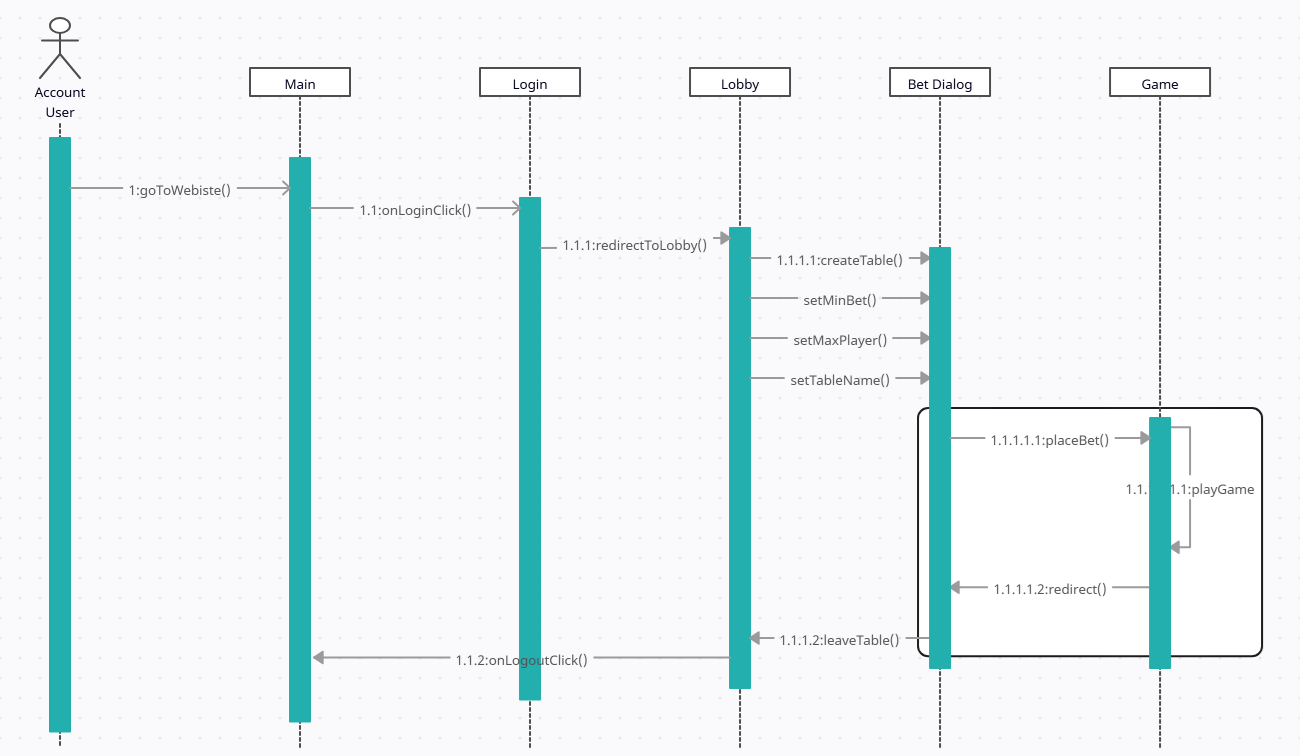
\includegraphics[width=1.0\linewidth]{figures/sequence.png}
    \caption{Sequence Diagram for a user playing the game}
    \label{fig:sequence}
\end{figure}

\noindent Figure \ref{fig:sequence} shows a sequence diagram for the user signing in and playing the game. The user starts at the landing page, logs in, is directed to the lobby, then either creates or joins a table, and then enters a loop in which the user keeps putting a bet in and playing the game until they are done and want to leave that table. 

\subsubsection{Sprint 2 Retrospective}
In this sprint we realized multiple things including the importance of planning stories. We were fortunate that we planned our stories based on core components of the app. Sprint 1 was focused on the model components of the app, allowing us to build all the of the social aspects of the app on top of the existing model components. Additionally, we realized the importance of having the ``main" branch be the most current working version of our project. Each member should push to their branch and then move it to main so that everyone else pulls from main rather than pulling from each other. This ensures that main is always up to date and compiles. We also switched our database from MySQL to Firebase. This was a good switch as we were having a lot of trouble with MySQL and Firebase was not only easy to use, but was also easy to covert to. 

\pagebreak

\subsection{Sprint 3}

\subsubsection{Plan}

\noindent After our last sprint we only had a few stories left to do that centered on admin privileges, table messaging, and full multiplayer functionality.

\subsubsection{Sprint 3 Stories}

\begin{table}[!hbt]
\centering
\caption{Overview for sprint 3}
\label{tab: overview for sprint 3}
\begin{tabular}{|c|c|c|c|c|}
\hline
\textbf{ID} & \textbf{Name}                                                       & \textbf{Points} & \textbf{Contributor} & \textbf{Status}                 \\ \hline
S6          & Remove Friend                                                       & 1               & Jenna                & {\color[HTML]{32CB00} Accepted} \\ \hline
S12         & Join Game                                                           & 2               & Chris                & {\color[HTML]{32CB00} Accepted} \\ \hline
S15         & Change Ace Value                                                    & 1               & Callie               & {\color[HTML]{32CB00} Accepted} \\ \hline
S17 & \begin{tabular}[c]{@{}c@{}}Send Chat \\ to Table\end{tabular} & 2 & Callie & {\color[HTML]{32CB00} Accepted} \\ \hline
S24         & Reset Password                                                      & 2               & Jenna                & {\color[HTML]{32CB00} Accepted} \\ \hline
S25         & Modify Profile                                                      & 2               & Emma                 & {\color[HTML]{32CB00} Accepted} \\ \hline
T5          & \begin{tabular}[c]{@{}c@{}}User info for \\ Admin\end{tabular}      & 1               & Jenna / Emma         & N/A                             \\ \hline
T6          & \begin{tabular}[c]{@{}c@{}}Refactor for \\ Multiplayer\end{tabular} & 1               & Chris                & N/A                             \\ \hline
\end{tabular}
\end{table}

\noindent Table \ref{tab: overview for sprint 3} shows the stories and technical tasks that were planned for sprint 3. We added more technical tasks to track work done not directly related to user stories. T5 has 2 contributors because both Jenna and Emma thought it was best to co-create an admin page so that they each were working on the same page when they got to their respective stories. T6 was to track the work that Chris put in while trying to refactor the game to support multiplayer.\\

\noindent \textbf{Individual Speeds and Cycle times}

\begin{table}[!hbt]
\centering
\caption{Individual metrics for sprint 3}
\label{tab: sprint 3 individual metrics}
\begin{tabular}{|c|c|c|c|c|}
\hline
\textbf{Name} &
  \textbf{\begin{tabular}[c]{@{}c@{}}Points\\ Attempted\end{tabular}} &
  \textbf{\begin{tabular}[c]{@{}c@{}}Points\\ Completed\\ (Speed)\end{tabular}} &
  \textbf{\begin{tabular}[c]{@{}c@{}}Work \\ (hrs)\end{tabular}} &
  \textbf{\begin{tabular}[c]{@{}c@{}}Cycle\\ (hrs/pts)\end{tabular}} \\ \hline
Chris  & 3 & 3 & 56 & 18.67 \\ \hline
Jenna  & 5 & 5 & 10 & 2     \\ \hline
Callie & 3 & 3 & 15 & 5     \\ \hline
Emma   & 3 & 3 & 11 & 3.67  \\ \hline
\end{tabular}
\end{table}

\noindent Table \ref{tab: sprint 3 individual metrics} shows the individual work put into sprint 3. The most notable piece of data is Chris's work hours. The problem we had in sprint 3 was that our game was not multiplayer yet. Chris's task was to update the game to support multiplayer which we had thought wasn't going to be as difficult as it was. This point also illustrates our sprint 1 retrospective about our user stories being underestimated. Chris's work spent to points accomplished ratio (cycle) was very high.

\subsubsection{Sprint 3 Testing}

Here are the individual testing results for each member: 

\begin{table}[!hbt]
\centering
\caption{Sprint 3 testing coverage by main contributor}
\label{tab: sprint 3 testing}
\begin{tabular}{|ccc|}
\hline
\multicolumn{1}{|c|}{\textbf{File}} & \multicolumn{1}{c|}{\textbf{Statement Coverage (\%)}} & \textbf{Branch Coverage (\%)} \\ \hline
\multicolumn{3}{|c|}{\textbf{Chris}}                                                          \\ \hline
\multicolumn{1}{|c|}{CardDisplay}      & \multicolumn{1}{c|}{64.25}          & 61.37          \\ \hline
\multicolumn{1}{|c|}{\textbf{Average}} & \multicolumn{1}{c|}{\textbf{64.25}} & \textbf{61.37} \\ \hline
\multicolumn{3}{|c|}{\textbf{Jenna}}                                                          \\ \hline
\multicolumn{1}{|c|}{ManageFriends}    & \multicolumn{1}{c|}{94.1}           & 84.21          \\ \hline
\multicolumn{1}{|c|}{FriendsList}      & \multicolumn{1}{c|}{100}            & 100            \\ \hline
\multicolumn{1}{|c|}{UserList}         & \multicolumn{1}{c|}{100}            & 100            \\ \hline
\multicolumn{1}{|c|}{Auth}             & \multicolumn{1}{c|}{100}            & 100            \\ \hline
\multicolumn{1}{|c|}{\textbf{Average}} & \multicolumn{1}{c|}{\textbf{98.52}} & \textbf{96.05} \\ \hline
\multicolumn{3}{|c|}{\textbf{Callie}}                                                         \\ \hline
\multicolumn{1}{|c|}{AuthContext}      & \multicolumn{1}{c|}{100}            & 100            \\ \hline
\multicolumn{1}{|c|}{ChatContext}      & \multicolumn{1}{c|}{91.66}          & 66.66          \\ \hline
\multicolumn{1}{|c|}{Chat}             & \multicolumn{1}{c|}{83.33}          & 66.66          \\ \hline
\multicolumn{1}{|c|}{ChatBox}          & \multicolumn{1}{c|}{100}            & 100            \\ \hline
\multicolumn{1}{|c|}{List}             & \multicolumn{1}{c|}{80}             & 100            \\ \hline
\multicolumn{1}{|c|}{ChatList}         & \multicolumn{1}{c|}{88.09}          & 55.55          \\ \hline
\multicolumn{1}{|c|}{AddUser}          & \multicolumn{1}{c|}{84.33}          & 69.23          \\ \hline
\multicolumn{1}{|c|}{UserInfo}         & \multicolumn{1}{c|}{100}            & 100            \\ \hline
\multicolumn{1}{|c|}{TableChat}        & \multicolumn{1}{c|}{88.67}          & 66.66          \\ \hline
\multicolumn{1}{|c|}{\textbf{Average}} & \multicolumn{1}{c|}{\textbf{91.89}} & \textbf{80.53} \\ \hline
\multicolumn{3}{|c|}{\textbf{Emma}}                                                           \\ \hline
\multicolumn{1}{|c|}{AllUsers}         & \multicolumn{1}{c|}{100}            & 100            \\ \hline
\multicolumn{1}{|c|}{SelectedUser}     & \multicolumn{1}{c|}{100}            & 92.85          \\ \hline
\multicolumn{1}{|c|}{ManageUsers}      & \multicolumn{1}{c|}{95.23}          & 80             \\ \hline
\multicolumn{1}{|c|}{\textbf{Average}} & \multicolumn{1}{c|}{\textbf{98.41}} & \textbf{90.95} \\ \hline
\end{tabular}
\end{table}

\noindent Table \ref{tab: sprint 3 testing} shows the coverage report for the files created and updated in sprint 3. Note that the CardDisplay file is the front end for our app which has a lot of response checking from the backend that couldn't be covered from an invalid response scenario, thus the low coverage.

\pagebreak


\begin{figure}
    \centering
    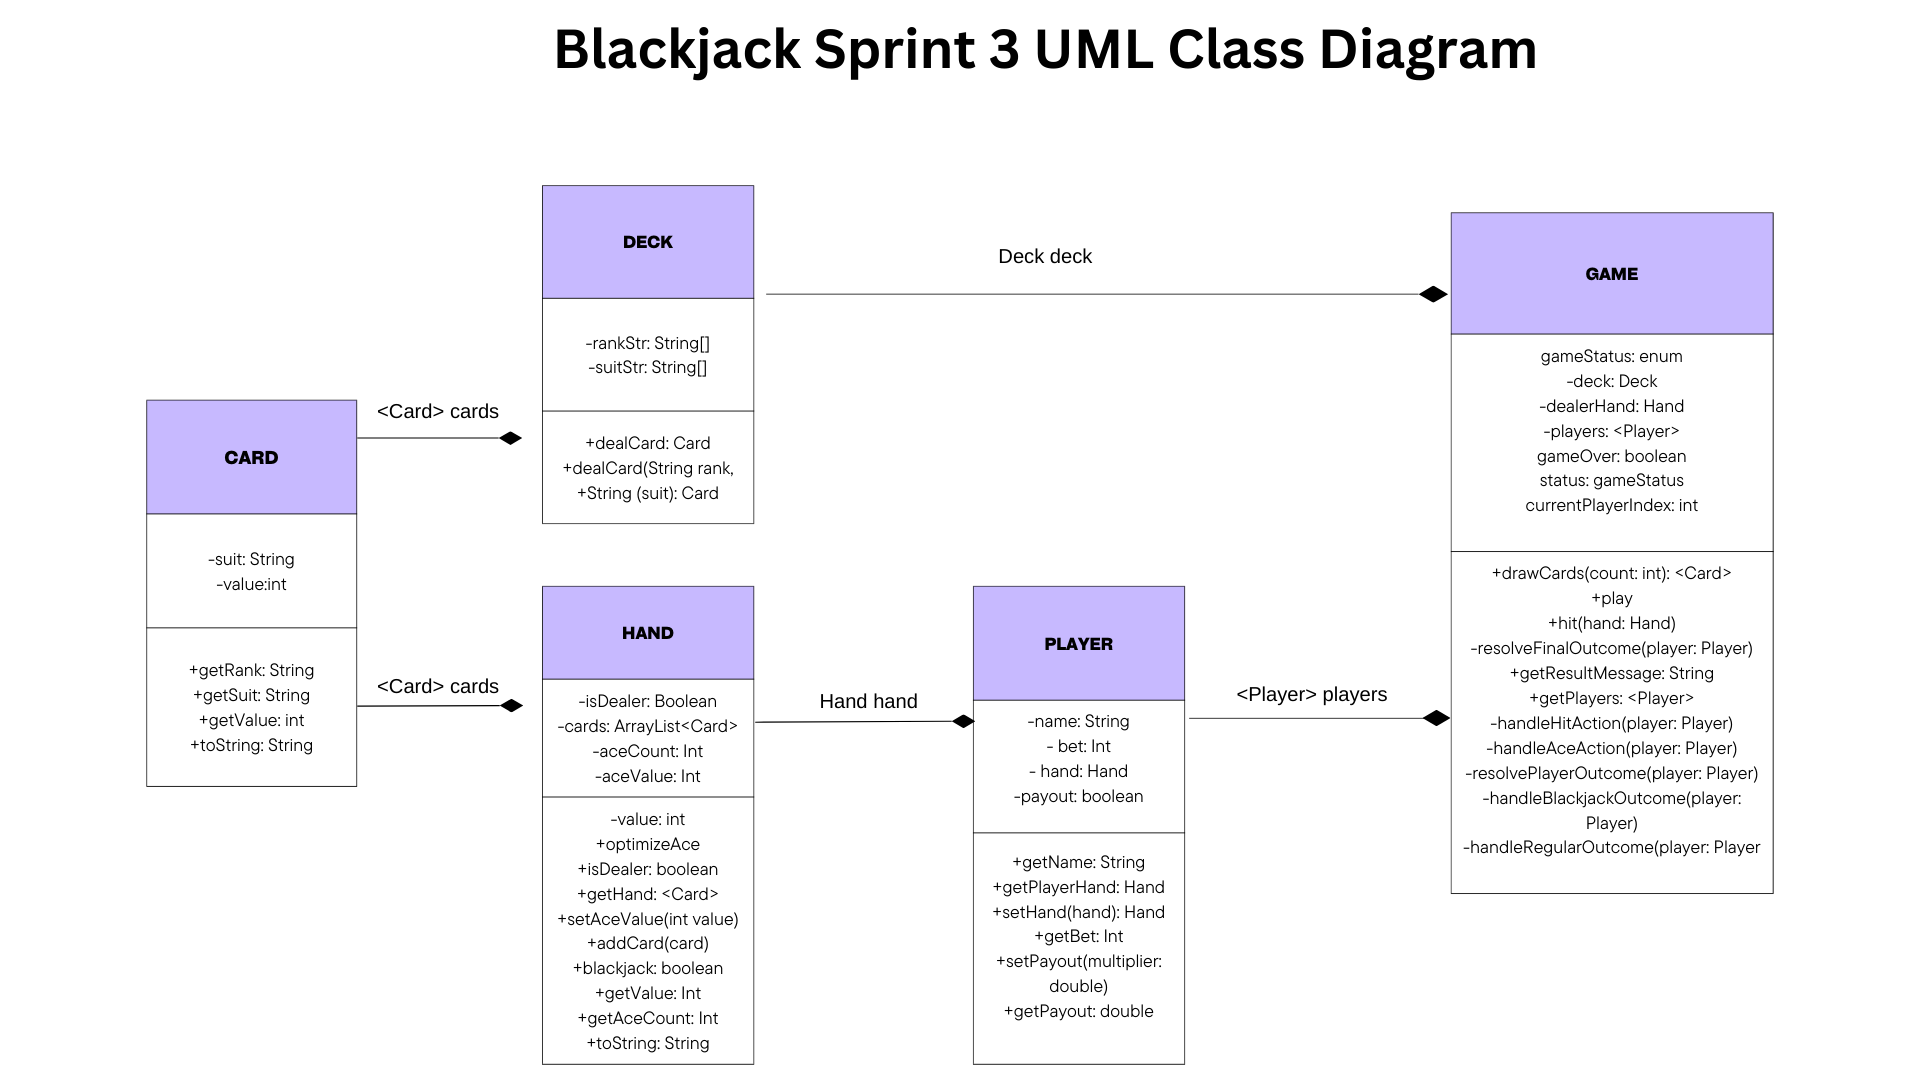
\includegraphics[width=1.0\linewidth]{figures/Sprint_3_UML_Diagram.png}
    \caption{Updated UML diagram for sprint 3}
    \label{fig:sprint 3 UML}
\end{figure}

\noindent Figure \ref{fig:sprint 3 UML} is our updated UML diagram for our model classes and their interactions.


\subsubsection{Sprint 3 Retrospective}
In this sprint we didn't have a lot of things left over from sprint 2. The big ticket item was getting multiplayer functionality done. That task was more challenging and time consuming than anticipated which is why Chris had so many hours for such few points this sprint, seen in Table \ref{tab: sprint 3 individual metrics}. The multiplayer aspect was under a 2 point story, which in hindsight should've been around 5-8 points. Other than that, we had a good pace and team dynamic which had been developing over the 3 sprints.


